
\section{Global Presentation of the Library}

\texttt{OpenMotion} is a open source library mainly aimed for real-time attitude estimation. Our approach is based on data fusion technics using only the output of a IMU (composed by a 3D gyroscope,  3D accelerometer and a 3D magnetometer). Among several sensor fusion algorithms proposed by the library, the user has the possibilities to choose the one that fits the best to his expectation according to its performance. 

However, we designed the library also as an academic tool. For this reason, we have chosen to implement for this library the most common family of methods. In previous works \cite{braudcomparison}, we proposed a comparative framework that allow us to observe the performance of this different methods in a quantitative manner. Thus, the user has in his disposition the code and and the performance study. This will help him to have a better understanding of the algorithms' mechanism and behavior. On the other hand, the user can use the library as a developing tool to design and create new sensor fusion algorithm. Moreover, he can compare his work directly with the available methods. For this paper,  2 references frames are used as follow:


\vspace{0.1cm}

\begin{itemize}
\item The North East Down (NED) frame $\{a\}$ system has its origin fixed at the (moving) object center of gravity. The $z$-axis points upward perpendicularly to the tangent plane of the ellipsoid, and the $x$-axis points towards true north (and not the magnetic north). The $y$-axis point towards east.

\vspace{0.1cm}

\item The object-fixed reference frame $\{c\}$ corresponding to the IMU device. It is a moving and rotating coordinate frame. 
\end{itemize}

\vspace{0.1cm}

For simplicity reasons, the library admit that all the components of the IMU belong to the same reference frame $\{c\}$ (ref figure \ref{Schema_situation}). It is a cyclopean approximation \cite{ouarti2008multimodal}. Moreover, the user has to interface the sends of data from the device to the library because the library does not take care of it. \texttt{OpenMotion} provide an estimation of the orientation of $\{c\}$ relative to $\{a\}$. The choice of the output type (quaternion, rotation matrix, euler angle) is also according to the user needs. 

\begin{figure}
\centering
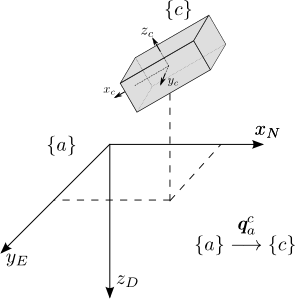
\includegraphics[scale=0.65]{images/Schema_situation.png}
\caption{Definition of the scene with 2 frame:  a fixed frame NED (North East Down) noted $\{a\}$ and a moving frame object noted $\{c\}$. \texttt{OpenMotion} will provide an estimate of the attitude of $\{c\}$ relative to $\{a\}$. }
\label{Schema_situation}
\end{figure}

We are also working on the establishment of a dynamic sensor calibration process on all component of the IMU. We insist on the dynamic aspect. Indeed, firstly, it allows  the library to be adaptable to any kind of IMU, but also to improve the performance without requesting some effort from the user.

